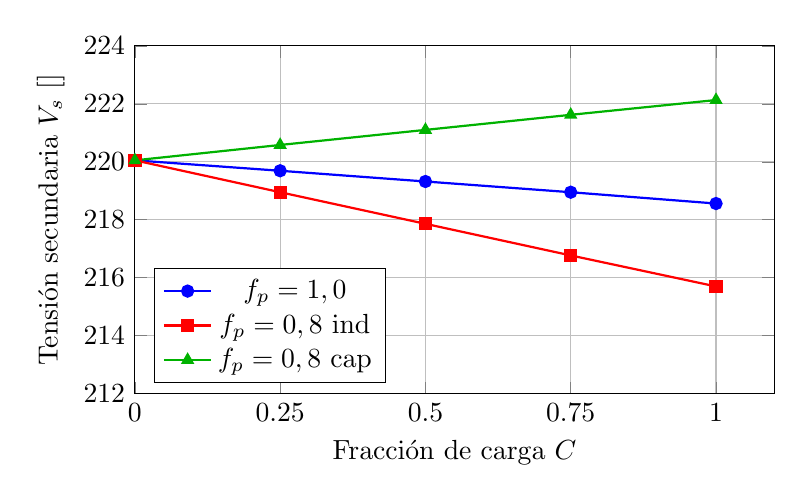
\begin{tikzpicture}
  \begin{axis}[
      xlabel={Fracción de carga $C$},
      ylabel={Tensión secundaria $V_s$ [\si{\volt}]},
      xmin=0, xmax=1.1,
      ymin=212, ymax=224,
      xtick={0, 0.25, 0.5, 0.75, 1},
      ytick={212, 214, 216, 218, 220, 222, 224},
      legend pos=south west,
      grid=major,
      width=0.8\textwidth,
      height=6cm
    ]
    % Carga resistiva (fp = 1)
    \addplot[color=blue, mark=*, thick] coordinates {
      (0, 220.05)
      (0.25, 219.69)
      (0.50, 219.32)
      (0.75, 218.95)
      (1.00, 218.56)
    };
    \addlegendentry{$f_p = 1,0$}

    % Carga inductiva (fp = 0.8 ind)
    \addplot[color=red, mark=square*, thick] coordinates {
      (0, 220.05)
      (0.25, 218.95)
      (0.50, 217.86)
      (0.75, 216.77)
      (1.00, 215.70)
    };
    \addlegendentry{$f_p = 0,8$ ind}

    % Carga capacitiva (fp = 0.8 cap)
    \addplot[color=green!70!black, mark=triangle*, thick] coordinates {
      (0, 220.05)
      (0.25, 220.58)
      (0.50, 221.10)
      (0.75, 221.62)
      (1.00, 222.13)
    };
    \addlegendentry{$f_p = 0,8$ cap}
  \end{axis}
\end{tikzpicture}
